\documentclass[a4paper,12pt]{scrartcl}
\usepackage[margin=2cm,bindingoffset=0cm]{geometry}
\usepackage{ucs}
\usepackage[utf8x]{inputenc}
\usepackage[ngerman]{babel}
\usepackage{fontenc}
%\usepackage[pdftex]{graphicx}
\usepackage{listings}
\usepackage{amssymb}
\usepackage{amsmath}
\usepackage{wasysym}
\usepackage{graphicx}
\usepackage[pdftex]{hyperref}
\author{
Verena Käfer (2551188),\\
Niklas Schnelle (2573250),\\
Peter Vollmer (2553704)}
\date{erstellt am 08.12.2010\\
Version: 1.0}
\title{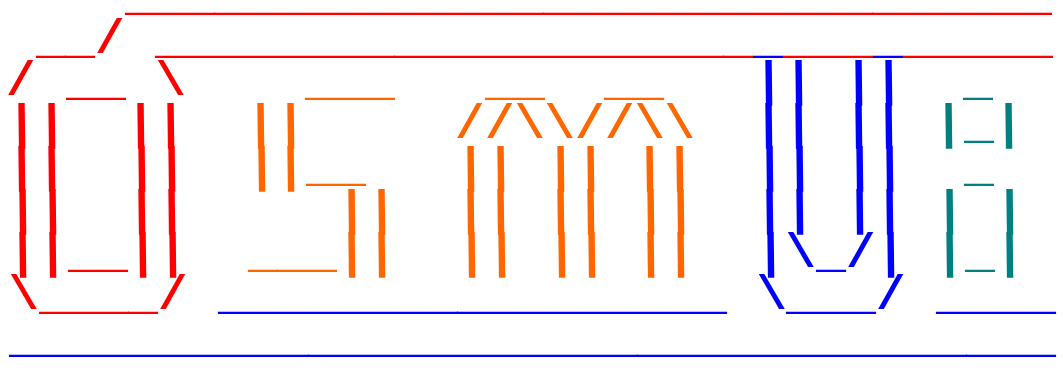
\includegraphics[width=15cm]{../projektplan/Logo_Osmui.png} \\ 
Entwurf von OsmUi}

\begin{document}
\maketitle
\newpage
\tableofcontents
\newpage

\section{Einleitung}
Die folgenden Abschnitte beschreiben den Entwurf und die Architektur von OsmUi.
\subsection{Das Software-System}
OsmUi stellt eine Benutzeroberfläche für das Kommandozeilen-Tool Osmosis dar. Die Implementierung erfolgt in Java, die Oberfläche wird mit Swing realisiert. Für die graphische Darstellung der Pipelines wird auf JGraph zurückgegeriffen. Die Pipelines werden entweder in xml-Dateien oder in smu-Dateien gespeichert.
\subsection{Entwurfsprinzipien}

\subsection{Überblick über den Entwurf}
In den folgenden Abschnitten werden zuerst die Architektur (Kapitel 2) und dann die einzelnen Komponenten (Kapitel 3) beschrieben. Die genaue Dokumentation der Klassen und Methoden erfolgt direkt im Programm als JavaDoc. Desweiteren soll dieses Dokument, die Entwurfsentscheidungen dokumentieren.

\section{Architektur}
\subsection{Komponentenübergreifende Funktionen}

\section{Komponenten}

\subsection{Komponente: XYZ}
\subsubsection{Schnittstelle}
\subsubsection{Protokoll}
\subsubsection{Verhalten}
\subsubsection{Interne Realisierung}
\subsubsection{Realisierte Anforderungen}
\subsection{Verbindungen}

\section{Externe Schnittstellen}
\subsection{Dauerhafte Datenspeicherung}
\subsubsection{Datei/Datenbank: XYZ}
\subsection{Externer Zugriff}
\subsubsection{Schnittstelle: XYZ}

\appendix%

\section{Anhang}

\section{Literatur zum Entwurf}
\subsection{Entwurf}
\subsection{Entwurfsmuster}

\end{document}